\documentclass{beamer}
\usepackage{amsmath}
\usepackage{amssymb}
%\usepackage{asymptote}
\usepackage{calc}
%\usepackage{caption}
%\usepackage{chemfig}
\usepackage{color}
\usepackage{commath}
%\usepackage{enumitem}
\usepackage[c]{esvect}
%\usepackage{etoolbox}
\usepackage{fancyhdr}
%\usepackage{float}
%\usepackage{fontspec}    %fontspec only works with xetex and luatex.
%\usepackage{fp}
\usepackage{geometry}
\usepackage{graphicx}
\usepackage{lastpage}
%\usepackage{listings}
%\usepackage{luacode}
\usepackage{mathtools}
%\usepackage{mhchem}
%\usepackage{pgfplots}
%\usepackage{setspace}
\usepackage{siunitx}
%\usepackage{tcolorbox}
%\usepackage{tikz}

\title{Visualizing Data using t-SNE}
\author{Taran Lynn, Xiaoli Yang, Xiaoxin Chen}

\begin{document}
\maketitle

\begin{frame}
  \frametitle{Data Visualization and Manifold Learning}
\end{frame}

\begin{frame}
  \frametitle{Stochastic Neighbor Embedding (SNE)}
  \framesubtitle{Spring Metaphor}

  \begin{figure}
    \centering
    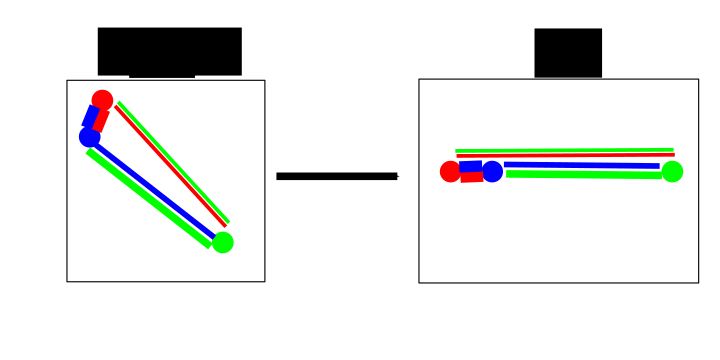
\includegraphics[width=\linewidth]{images/spring.png}
  \end{figure}
\end{frame}

\begin{frame}
  \frametitle{Stochastic Neighbor Embedding (SNE)}
  \framesubtitle{What is $p_{j|i}$?}

  \begin{figure}
    \centering
    \includegraphics[width=0.6\linewidth]{images/gauss/gauss.png}
  \end{figure}
\end{frame}

\begin{frame}
  \frametitle{Stochastic Neighbor Embedding (SNE)}
  \framesubtitle{Gradient Descent Optimization}
\end{frame}

\begin{frame}
  \frametitle{Stochastic Neighbor Embedding (SNE)}
  \framesubtitle{Determining $\sigma_i$}

  \begin{center}
    \small
    
    \begin{tabular}{ll}
      Perplexity & Smooth approximation of number of neighbors\\
      & $Perp(P_i) = 2^{H(P_i)}$\\
      \hline
      Shannon Entropy & Information present in probability space\\
      & $H(P_i) = -\sum_j p_{j|i} \log_2{p_{j|i}}$\\
    \end{tabular}
  \end{center}
  
  \begin{figure}
    \centering
    \includegraphics[height=0.6\textheight]{images/perp/perp.png}
  \end{figure}
\end{frame}

\begin{frame}
  \frametitle{Problems with SNE}

  \begin{itemize}
  \item Computational inefficiency

  \item Overcrowding
  \end{itemize}
\end{frame}

\end{document}
